\documentclass[a4paper,12pt]{extarticle}
\usepackage[utf8x]{inputenc}
\usepackage[T1,T2A]{fontenc}
\usepackage[russian]{babel}
\usepackage{hyperref}
\usepackage{indentfirst}
\usepackage{listings}
\usepackage{color}
\usepackage{here}
\usepackage{array}
\usepackage{multirow}
\usepackage{graphicx}

\usepackage{caption}
\renewcommand{\lstlistingname}{Программа} % заголовок листингов кода

\bibliographystyle{ugost2008ls}

\usepackage{listings}
\lstset{ %
extendedchars=\true,
keepspaces=true,
language=C,						% choose the language of the code
basicstyle=\footnotesize,		% the size of the fonts that are used for the code
numbers=left,					% where to put the line-numbers
numberstyle=\footnotesize,		% the size of the fonts that are used for the line-numbers
stepnumber=1,					% the step between two line-numbers. If it is 1 each line will be numbered
numbersep=5pt,					% how far the line-numbers are from the code
backgroundcolor=\color{white},	% choose the background color. You must add \usepackage{color}
showspaces=false				% show spaces adding particular underscores
showstringspaces=false,			% underline spaces within strings
showtabs=false,					% show tabs within strings adding particular underscores
frame=single,           		% adds a frame around the code
tabsize=2,						% sets default tabsize to 2 spaces
captionpos=t,					% sets the caption-position to top
breaklines=true,				% sets automatic line breaking
breakatwhitespace=false,		% sets if automatic breaks should only happen at whitespace
escapeinside={\%*}{*)},			% if you want to add a comment within your code
postbreak=\raisebox{0ex}[0ex][0ex]{\ensuremath{\color{red}\hookrightarrow\space}},
texcl=true,
inputpath=listings,                     % директория с листингами
}

\usepackage[left=2cm,right=2cm,
top=2cm,bottom=2cm,bindingoffset=0cm]{geometry}

%% Нумерация картинок по секциям
\usepackage{chngcntr}
\counterwithin{figure}{section}
\counterwithin{table}{section}

%%Точки нумерации заголовков
\usepackage{titlesec}
\titlelabel{\thetitle.\quad}
\usepackage[dotinlabels]{titletoc}

%% Оформления подписи рисунка
\addto\captionsrussian{\renewcommand{\figurename}{Рисунок}}
\captionsetup[figure]{labelsep = period}

%% Подпись таблицы
\DeclareCaptionFormat{hfillstart}{\hfill#1#2#3\par}
\captionsetup[table]{format=hfillstart,labelsep=newline,justification=centering,skip=-10pt,textfont=bf}

%% Путь к каталогу с рисунками
\graphicspath{{fig/}}

%% Внесение titlepage в учёт счётчика страниц
\makeatletter
\renewenvironment{titlepage} {
 \thispagestyle{empty}
}
\makeatother


\begin{document}	% начало документа

% Титульная страница
\begin{titlepage}	% начало титульной страницы

	\begin{center}		% выравнивание по центру

		\large Санкт-Петербургский политехнический университет Петра Великого\\
		\large Институт компьютерных наук и технологий \\
		\large Кафедра компьютерных систем и программных технологий\\[6cm]
		% название института, затем отступ 6см
		
		\huge «Технологии программирования (Java)»\\[0.5cm] % название работы, затем отступ 0,5см
		\large Отчет по курсовой работе\\[0.1cm]
		\large Игра 2048 на Android\\[5cm]

	\end{center}


	\begin{flushright} % выравнивание по правому краю
		\begin{minipage}{0.25\textwidth} % врезка в половину ширины текста
			\begin{flushleft} % выровнять её содержимое по левому краю

				\large\textbf{Работу выполнил:}\\
				\large Симоновский Д. Л.\\
				\large {Группа:} 3530901/10001\\
				
				\large \textbf{Преподаватель:}\\
				\large Алексюк А. О.

			\end{flushleft}
		\end{minipage}
	\end{flushright}
	
	\vfill % заполнить всё доступное ниже пространство

	\begin{center}
	\large Санкт-Петербург\\
	\large \the\year % вывести дату
	\end{center} % закончить выравнивание по центру

\end{titlepage} % конец титульной страницы

\vfill % заполнить всё доступное ниже пространство


% Задание
\newcommand{\textunderline}[2]{\lower\baselineskip\vbox{\halign{##\cr \underline{#1} \hrulefill\cr \tiny{#2\\}\cr}}}

\begin{center} % выравнивание по центру

	\large ЗАДАНИЕ \\
	\large НА ВЫПОЛНЕНИЕ КУРСОВОГО ПРОЕКТА \\

\end{center}
Студенту группы \textunderline{3530901/10001}{Номер группы}\hspace{3mm}\textunderline{Симоновскому Даниилу Леонидовичу}{Фамилия, Имя, Отчество}
\textbf{ % Делаю шрифт жирным
	\begin{enumerate} % Делаю список
		\item Тема проекта: {\normalfont \underline{<<2048>>}}
		\item Срок сдачи законченного проекта: {\normalfont \underline{21.05.2022}}
		\item Исходные данные к проекту: {\normalfont \underline{IDE: Android Studio Chipmunk 2021.2.1}}
		\item Содержание пояснительной записки {\normalfont (перечень подлежащих разработке вопросов): введение, основная часть (текст программы, описание программы, испытания программы), заключение, список использованных источников.}
	\end{enumerate}
}
\vspace{2cm}
\textbf{Дата получения задания:} \underline{<<9>> апреля} 2022 г.

\vspace{5cm}

Руководитель\hfillАлексюк А.О.

Задание принял к исполнению \hfillСимоновский Д.Л.

\underline{<<9>> апреля} 2022 г.
\newpage

% Содержание
% Содержание
\renewcommand\contentsname{\centerline{Содержание}}
\tableofcontents
\newpage




\section{Цель работы}
Создать и протестировать игру 2048 на Android

\section{Правила игры}
\textbf{2048} - игра для одного человка. В ней путём свайпов (в оригинале нажатий на стрелочки) игрок может скинуть все плитки игрового поля в одну из 4 сторон. Если при сбрасывании две плитки одного номинала «налетают» одна на другую, то они превращаются в одну, номинал которой равен сумме соединившихся плиток. После каждого хода на свободной секции поля появляется новая плитка номиналом «2» (90\%) или «4» (10\%). Если при нажатии кнопки местоположение плиток или их номинал не изменится, то ход не совершается.

Если в одной строчке или в одном столбце находится более двух плиток одного номинала, то при сбрасывании они начинают соединяться с той стороны, в которую были направлены. Например, находящиеся в одной строке плитки (4, 4, 4) после хода влево превратятся в (8, 4), а после хода вправо — в (4, 8). Данная обработка неоднозначности позволяет более точно формировать стратегию игры.

За каждое соединение игровые очки увеличиваются на номинал получившейся плитки.

Игра заканчивается поражением, если после очередного хода невозможно совершить действие.

Игра заканчивается победой, если была достигнута клетка наминалом 2048

\section{Описания решения}
Приложение разделено на 2 пакета: \textit{<<core>>} и \textit{<<ui>>}. Изначально планировалось использовать модель <<Model-View-Controller>>, однако было принятно решение от неё отказаться в пользу упрощения чтения кода т.к. часть <<Controller>> добавляла слишком много лишней смысловой нагрузки.

\subsection{core}
Пакет <<core>> описывает саму логику работы игры, все перемещения, объединения цифр обрабатываются именно там. Пакет <<core>> содержит:
\begin{itemize}
\item Публичный enum \textbf{<<Direction>>}. Используется для передачи в основную часть информацию о направлении передвижения плиток.
\item Package-private class \textbf{<<Vector>>}. Используется для преобразования из не очень очевидного <<Direction>> в конкретные цифры перемещения по \textit{x} и \textit{y}
\item Публичный class \textbf{<<Coordinate>>}. Представляет из себя координаты на поле определенной клетки. Имеет в себе функции для взаимодействий с классом <<Vector>> (в частности сложение)
\item Публичный вложенный в <<Coordinate>> static class \textbf{<<Move>>}. Используется для того, чтоб передать перемещение фигуры из точки \textit{from} в точку \textit{to}, необходим для дальнейшей анимации.
\item Публичный class \textbf{<<Game>>}. В этом классе происходит вся логика предложения. Он содержит следующие публичные методы:
\subitem \textbf{doMove(Direction)} - совершает само перемещение фигур в направлении, переданном в Direction. Возвращает List из Move т.е. перемещения клеток 
\subitem \textbf{spawnSquare()} - создает на поле новую фигуру (90\% - 2, 10\% - 4) и возвращает Pair из Coordinate с местом, где появилась и фигура, и цифры на фигре. Или null, в случае, если места на поле нет.
\subitem \textbf{gameIsLost()} - возвращает информацию о том, проиграна ли игра.
\subitem \textbf{getScore()} - возвращает текущий счет игры.
\end{itemize}

\subsection{ui}
Пакет <<ui>> является смесью из View и Controller, в нем происходит отображение всего происходящего и обработка нажатий кнопок и свайпов. Этот пакет содержит:
\begin{itemize}
\item Публичный class \textbf{<<OnSwipeTouchListener>>}. Этот класс был взят из открытых источников и используется для получения направления свайпов.
\item Публичный class \textbf{<<Board>>}. Этот класс наследуется от View и представляет собой поле, отображаемое на экане телефона. В нем присутсвует метод для преобразования из координаты, полученной из core в координату на экране телефона, для дальнейшей отрисовки.
\item Публичный class \textbf{<<Square>>}. Этот класс наследуется от View и представляет собой плитку, отображаемую на экране телефона. Меняет цветплитки и цвет шрифта в зависимоти от цифры на плитке (цвета взяты из открытого репозитория создателя игры).
\item Публичный class \textbf{<<GameActivity>>}. В этом классе происходит всё, что отвечает за визуальную часть игры:
\subitem \textbf{onCreate()} - метод, вызываемый при открытие приложения. В началае устанавливается xml файл (activity\_game.xml), который хранит расположение всех элементов на экране. После этого я по id получаю доступ к элементам с экрана, которые меня интересуют. Далее присходит настройка кнопок: я добавляю каждой кнопке слушателя, чтоб при её нажатии что-то происходило (кнопка quit - выход, кнопка restart - перезапуск), добавляет слушателя на объект swipeDetector, чтоб вызывать функцию doIteration в направлении свайпа. После чего вызывается метод старт.
\subitem \textbf{start()} - метод для начала игры. Устанавливает таймер на 0 и запускает его, устанавливает счет на 0, пересоздает доску, создает первую плику.
\subitem \textbf{doIteration()} - метод, вызываемый при свайпе на экране. С анимацей перемещает все плитки в направлении свайпа, потом с анимацией объединяет необходимые. После всего этого спавнит новую плитку, вызывает обновление счёта и проверяет игру на победу/поражение (при необходимости вызывает метод endGame).
\subitem \textbf{endGame(String)} - останавливает таймер, выводит на экран текст, переданный в функцию.
\subitem \textbf{restart()} - метод, вызываемый при нажатии кнопки restart, делает приготовления, после чего вызывает метод start
\end{itemize}

\section{Внешний вид приложения}
На данных скриншотах видно пустое поле и поле с большим числом плиток разного цвета, а также меню проигрыша:

\begin{figure}[h]
	\begin{center}
		\begin{minipage}[h]{0.4\linewidth}
			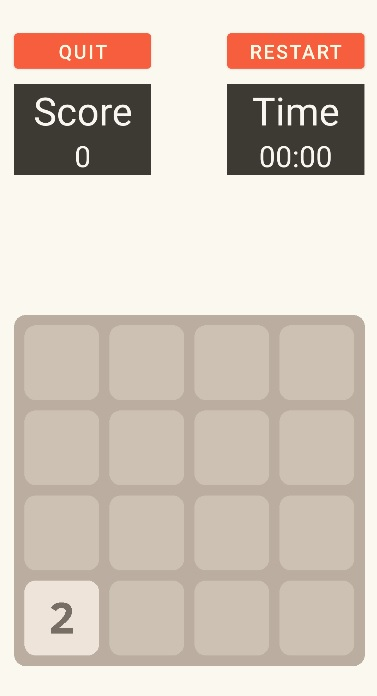
\includegraphics[width=1\linewidth]{empty field}
			\caption{Пустое поле} %% подпись к рисунку
			\label{fig:emptyField} %% метка рисунка для ссылки на него
		\end{minipage}
		\hfill
		\begin{minipage}[h]{0.4\linewidth}
			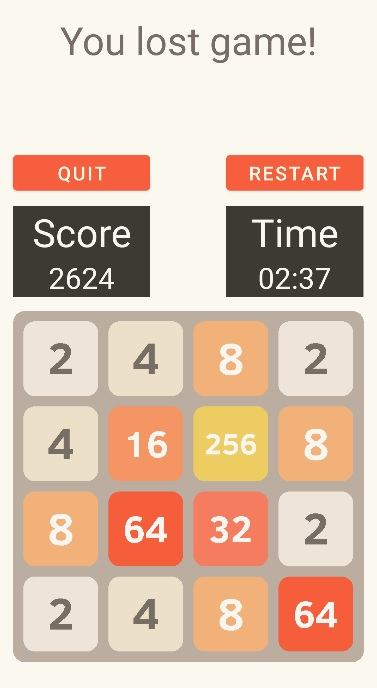
\includegraphics[width=1\linewidth]{colors}
			\caption{Поле с плитками}
			\label{ris:colors}
		\end{minipage}
	\end{center}
\end{figure}

\section{Тестирование}
Были сделаны Unit тесты для core части в количестве 10 штук, что дает 90\% покрытия. Присутсвуют как и обычные тесты, так и те, которые возникли в процессе дебагинга. Смысла отдельно рассматривать каждый тест нет, для подробного изучения см. репозиторий на гитхаб.


\section{Выводы}
В ходе проделанной работы была создана игра 2048 на Android, которая ничуть не уступает оригиналу. Были разработаны тесты, которые проверяют правильность работы кода.

Исходный код проекта можно найти по ссылке на \underline{\href{https://github.com/DafterT/ProgrammingLabSummer2022Task3}{GitHub}}

\section{Источники}

\begin{itemize}
\item \href{https://github.com/gabrielecirulli/2048}{\underline{github.com}} - репозиторий с исходным кодом оригинального 2048
\item \href{https://ru.wikipedia.org/wiki/2048\_(%D0%B8%D0%B3%D1%80%D0%B0)}{\underline{wikipedia.org}} - описание правил игры 2048
\end{itemize}
\end{document}
